
\chapter{Plots}
\label{ch:plots}
\newgeometry{inner=2.5cm,outer=2.5cm,bottom=2.5cm,top=0.5cm}
\begin{figure}
\makebox[\textwidth][c]{
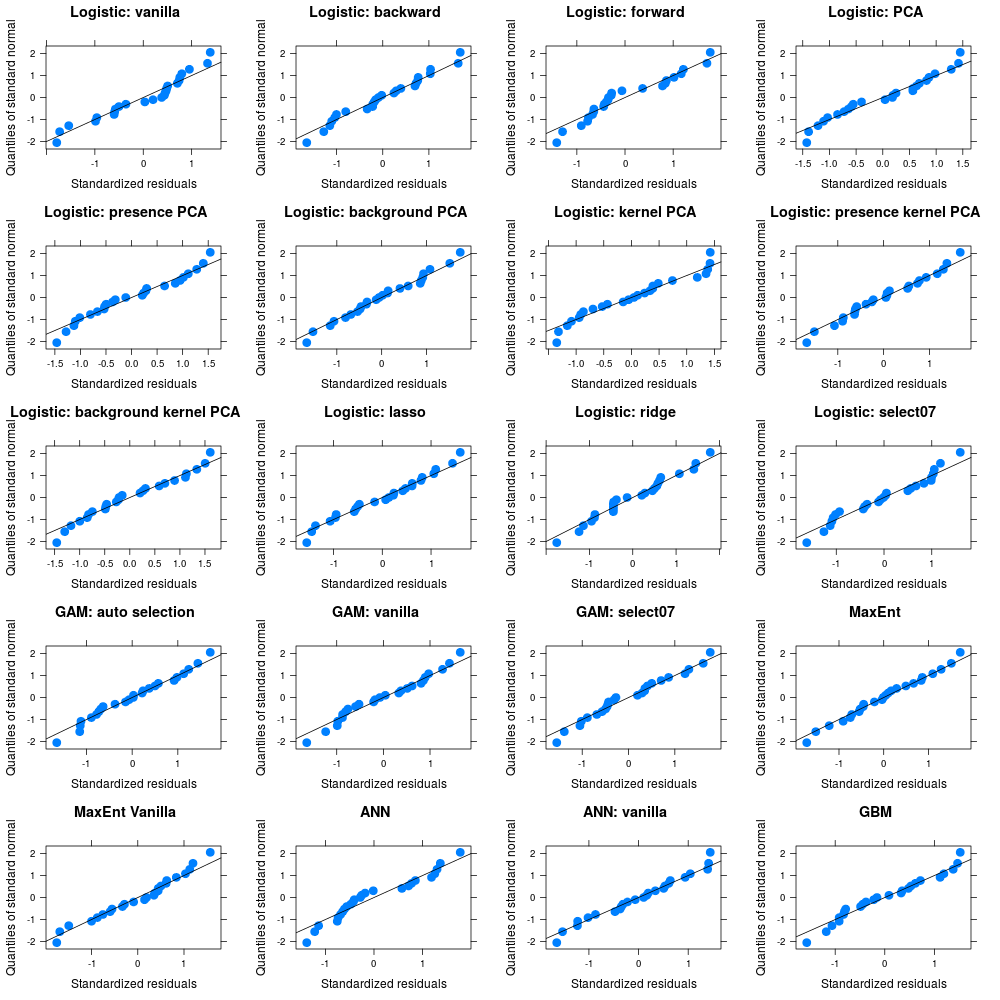
\includegraphics[scale=.7]{Plots/ResidualPlotsGLS.png}
}
\caption{\label{fig:ResidualGLSAll}QQ-plot of the residuals of the GLS model for the models fitted on all the variables.}
\end{figure}


\begin{figure}
\makebox[\textwidth][c]{
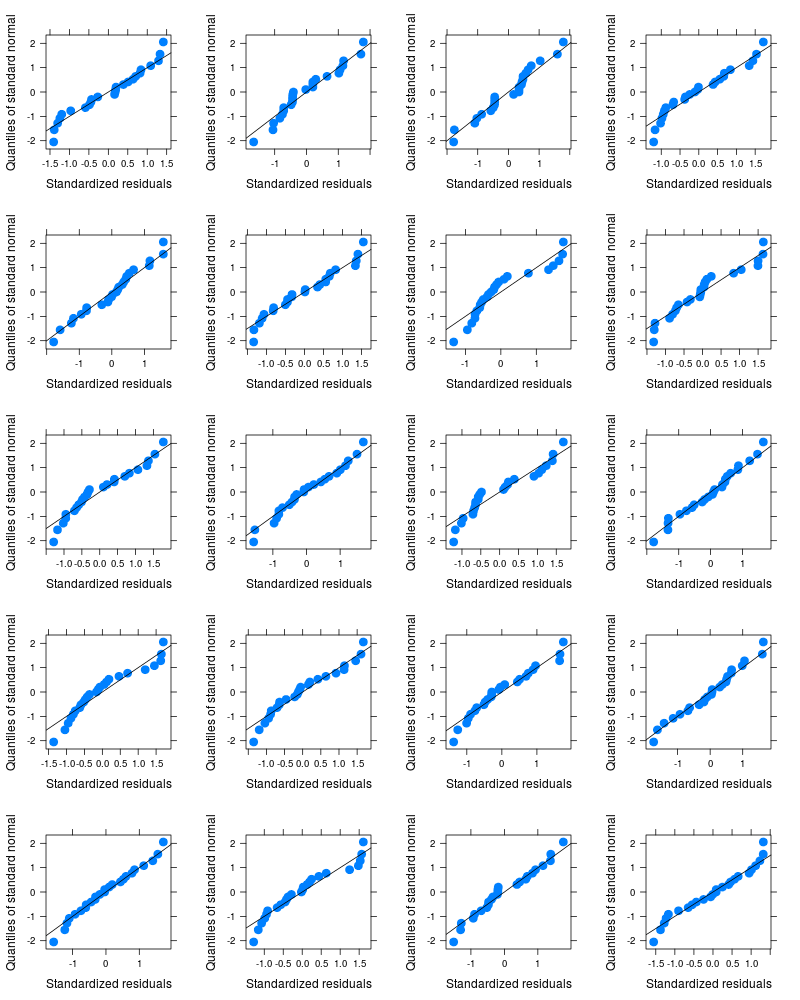
\includegraphics[scale=.7]{Plots/ResidualPlotGLSBio.png}
}
\caption{\label{fig:ResidualGLSBio}QQ-plot of the residuals of the GLS model for the models fitted with only the bioclimatic variables.}
\end{figure}

\begin{figure}
\makebox[\textwidth][c]{
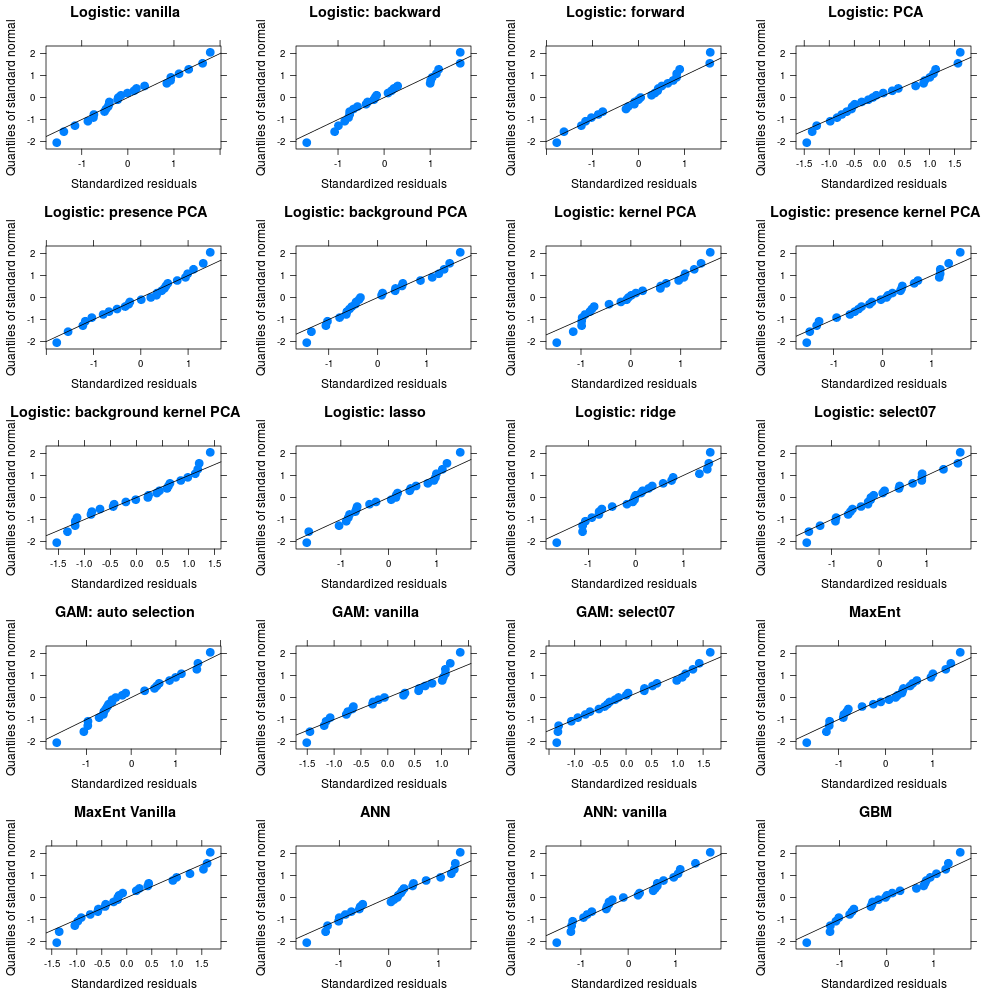
\includegraphics[scale=.7]{Plots/ResidualPlotGLSDiff.png}
}
\caption{\label{fig:ResidualGLSDiff}QQ-plot of the residuals of the GLS model for difference between the models fitted on the all variables versus only the bioclimatic variables.}
\end{figure}

\restoregeometry